\documentclass[xcolor=x11names]{beamer}

\usetheme{EIS}

\usepackage{graphicx}
\usepackage{hyperref}
\usepackage{xspace}
\usepackage{attrib}
\usepackage{booktabs}
\usepackage{color}
\usepackage{ragged2e}
\usepackage{multicol}
\usepackage{tikz}
\usetikzlibrary{arrows,shapes,backgrounds}
\usepackage{fontspec}
\defaultfontfeatures{Ligatures=TeX}
\newfontfeature{Microtype}{protrusion=default;expansion=default;}
%\setmainfont[Microtype]{Computer Modern Sans}
\usepackage{microtype}
%\setmainfont{Linux Libertine}
%\setsansfont{Linux Biolinum}

\usepackage{array}
\newcolumntype{L}[1]{>{\raggedright\let\newline\\\arraybackslash\hspace{0pt}}m{#1}}
\newcolumntype{C}[1]{>{\centering\let\newline\\\arraybackslash\hspace{0pt}}m{#1}}

\newcommand{\work}[1]{\textit{#1}\xspace}

\setbeamertemplate{navigation symbols}{}

\usepackage[english]{babel}

\renewcommand*{\thefootnote}{\ensuremath{\ast}}

\def\dunyazad/{\textit{Dunyazad}}
\def\minstrel/{\textit{Minstrel}}
\def\skald/{\textit{Skald}}
\def\problemplanets/{\textit{Problem Planets}}
\def\facade/{\textit{Fa\c{c}ade}}


\title[AI for Understanding Narrative Choices] 
{%
Artificial Intelligence as a Tool for Understanding Narrative Choices%
}

\author[Mawhorter]
{%
  Peter~Mawhorter
}

\institute[UCSC]
{%
  Department of Computer Science \\
  University of California Santa Cruz
}

\date[2016-3-3]
{%
  March 3rd, 2016
}

\begin{document}

\begin{frame}
  \titlepage
\end{frame}

\begin{frame}{Narrative Choices}
\begin{center}
  \includegraphics[width=0.8\textwidth]{res/cyoa-covers.jpg}
\end{center}
\end{frame}

\begin{frame}{Narrative Choices}
\begin{center}
  \includegraphics[height=0.8\textheight]{res/cave-of-time-cover.jpg}
  \hspace*{2em}
  \includegraphics[height=0.8\textheight]{res/cave-of-time-warning.jpg}
\end{center}
\end{frame}

\begin{frame}{Motivation}
\begin{center}
  \includegraphics[width=0.95\textwidth]{res/mass-effect-cyoa.jpg}
\end{center}
\end{frame}

\begin{frame}{Motivation: Understanding Popular Culture}
\begin{center}
  \includegraphics[width=\textwidth]{res/media-use-by-type.png} \\
  \vspace{1em}
  \tiny%
  Graph from the Growing Up With Media longitudinal study 2006--2008; participants were 10--15 years old. \\
  \vspace{1em}
  Published by the Center for Innovative Public Health Research \\
  \vspace{1em}
  \url{https://innovativepublichealth.org/bulletins/growing-up-with-media-media-use-patterns/}
\end{center}
\end{frame}

\begin{frame}{Motivation: Understanding Literature...}
\begin{center}
  \includegraphics[height=0.8\textheight]{res/to-kill-a-mockingbird-cover.jpg}
  \hspace*{2em}
  \includegraphics[height=0.8\textheight]{res/literary-devices.jpg}
\end{center}
\end{frame}

\begin{frame}{Motivation: Understanding Games?}
\begin{center}
  \includegraphics[height=0.45\textheight]{res/journey-title.png}
  \hspace*{1em}
  \includegraphics[height=0.45\textheight]{res/that-dragon-cancer.png}
  \vspace{1em}
  What can we say about how to understand and interpret these?
\end{center}
\end{frame}

\begin{frame}{Motivation: AI and Society}
\begin{center}
  \includegraphics[height=0.4\textheight]{res/siri.png}
  \hspace*{1em}
  \includegraphics[height=0.4\textheight]{res/facebook-ai-research.png}
  \hspace*{1em}
  \includegraphics[height=0.4\textheight]{res/facade-title.png} \\
  \vspace{1em}
  If AI is enabling new media and modes of communication, can it also help us understand them?
\end{center}
\end{frame}

\begin{frame}{My Thesis}
  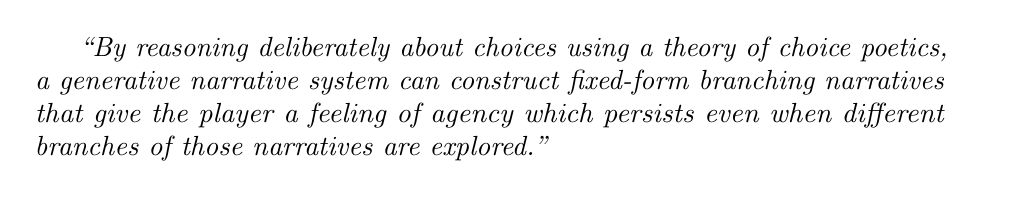
\begin{tikzpicture}
    \node(t)[text width=\textwidth] at (0,0) {%
      \parbox{0.95\textwidth}{
  \justifying%
  \itshape%
``By reasoning deliberately about choices using a theory of choice poetics, a generative narrative system can construct fixed-form branching narratives that give the player a feeling of agency which persists even when different branches of those narratives are explored.''%
    }};
  \end{tikzpicture}
\end{frame}

\begin{frame}{My Thesis}
  \vspace*{-0.05ex}%
  \hspace*{-0.25ex}%
  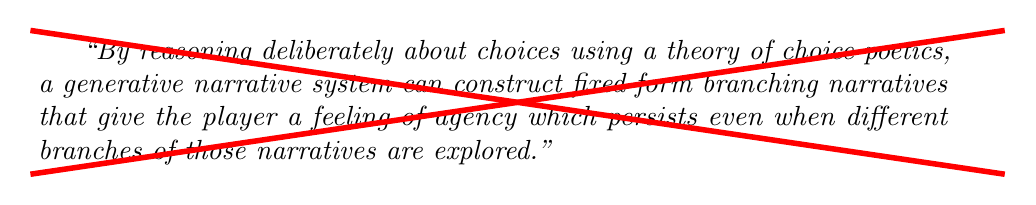
\begin{tikzpicture}
    \node(t)[text width=\textwidth] at (0,0) {%
      \parbox{0.95\textwidth}{
  \justifying%
  \itshape%
``By reasoning deliberately about choices using a theory of choice poetics, a generative narrative system can construct fixed-form branching narratives that give the player a feeling of agency which persists even when different branches of those narratives are explored.''%
    }};
    \draw[color=red,line width=2pt] (t.north west) -- (t.south east);
    \draw[color=red,line width=2pt] (t.south west) -- (t.north east);
  \end{tikzpicture}
\end{frame}

\begin{frame}{My Thesis}
  \justifying
  \itshape
  ``The simultaneous development of a theory for analyzing choice poetics and a system that operationalizes said theory to generate narrative choices provides benefits for both the system and the theory. This novel combination of critical and technical concerns has resulted in an original generative system as well as an analysis framework for understanding choices in terms of player goals.''
\end{frame}

\begin{frame}{My Thesis}
  \justifying
  \itshape
  ``The simultaneous development of a theory for analyzing choice poetics and a system that operationalizes said theory to generate narrative choices provides benefits for both the system and the theory.This \textbf{novel combination of critical and technical concerns} has resulted in an original generative system as well as an analysis framework for understanding choices in terms of player goals.''
\end{frame}

\begin{frame}{My Thesis}
  \justifying
  \itshape
  ``The simultaneous development of a theory for analyzing choice poetics and a system that operationalizes said theory to generate narrative choices provides benefits for both the system and the theory. This novel combination of critical and technical concerns has resulted in \textbf{an original generative system} as well as an analysis framework for understanding choices in terms of player goals.''
\end{frame}

\begin{frame}{My Thesis}
  \justifying
  \itshape
  ``The simultaneous development of a theory for analyzing choice poetics and a system that operationalizes said theory to generate narrative choices provides benefits for both the system and the theory. This novel combination of critical and technical concerns has resulted in an original generative system as well as \textbf{an analysis framework for understanding choices in terms of player goals}.''
\end{frame}

\begin{frame}{Outline}
  \begin{itemize}
    \item Motivation
    \item \textbf{Inspiration: \skald/ and \problemplanets/}
    \item \textbf{Methodology}
    \item \textbf{Related Work}
    \item \textbf{Theory: Choice Poetics}
    \item \textbf{Application: \dunyazad/}
    \item \textbf{Results: Options}
    \item \textbf{Results: Outcomes}
    \item \textbf{Conclusions}
  \end{itemize}
\end{frame}

\begin{frame}{\minstrel/}
  \justifying
  \setlength{\parindent}{1.5em}
  \itshape
  It was the spring of 1089, and a knight named Lancelot returned to Camelot from elsewhere. Lancelot was hot tempered. Once, Lancelot had lost a joust. Because he was hot tempered, Lancelot wanted to destroy his sword. Lancelot struck his sword. His sword was destroyed.

  One day, a lady of the court named Andrea wanted to have some berries\ldots
\end{frame}

\begin{frame}{\minstrel/}
  \vfill
  \begin{itemize}\addtolength{\itemsep}{0.5\baselineskip}
    \item Case-based story generation.
    \item Models human creativity through `Transform-Recall-Adapt Methods' (TRAMs).
    \item Manages story construction via `Author-Level Plans' (ALPs).
  \end{itemize}
  \vfill
  \centering
  \tiny ``\textsc{Minstrel}: A Computer Model of Creativity and Storytelling'' (Turner 1993)
\end{frame}

\begin{frame}{\skald/}
  \vfill
  \begin{itemize}\addtolength{\itemsep}{0.5\baselineskip}
    \item A rational reconstruction of \minstrel/.
    \item Focused on the TRAMs for imaginative recall.
    \item We experimented with different TRAM and ALP setups.
  \end{itemize}
  \vfill
  \centering
  \tiny ``Experimental Results from a Rational Reconstruction of Minstrel'' (Tearse et al. 2011) \\
  \tiny ``Lessons Learned from a Rational Reconstruction of Minstrel'' (Tearse et al. 2012) \\
  \tiny ``Skald: Minstrel Reconstructed'' (Tearse et al. 2014) \\
\end{frame}

\begin{frame}{\skald/: Experiments}
  \begin{itemize}\addtolength{\itemsep}{0.5\baselineskip}
    \item Results:
    \begin{itemize}\addtolength{\itemsep}{0.5\baselineskip}
      \vspace{0.5\baselineskip}
      \item TRAM configurations can trade coherence against variety.
      \item Modified boredom and TRAM selection can reduce search effort but also creativity.
    \end{itemize}
  \end{itemize}
  \vspace{1ex}
  \begin{tabular}{p{0.45\textwidth} p{0.45\textwidth}}
  \scriptsize
  \centering
  TRAM experiment: \newline
  \begin{tabular}{r c c}
      \toprule
      measure & orig. & mod. \\
      \midrule
      coherence & 35\% & 92\%  \\
      unique & 69 & 12 \\
      variation & 6.9 & 3.1  \\
      \bottomrule
  \end{tabular}
  &
  \scriptsize
  \centering
  Full system experiment: \newline
  \begin{tabular}{r c c}
      \toprule
      measure & orig. & mod. \\
      \midrule
      direct matches & 59\% & 72\% \\
      TRAMs tried & 13.8 & 7.7  \\
      TRAMs used & 2.4 & 1.4  \\
      \bottomrule
  \end{tabular} \newline
\end{tabular}
\end{frame}

\begin{frame}{\problemplanets/}
  \begin{itemize}\addtolength{\itemsep}{0.5\baselineskip}
    \item A project to use \skald/ to build interactive vignettes.
    \item Vignettes would educate about climate-change related issues.
    \item The case library required delicate balancing.
    \item Efforts to ensure coherence resulted in complex ALPs.
    \item The placement of choices to add interactivity was static.
  \end{itemize}
\end{frame}

\begin{frame}{\problemplanets/}
  \begin{itemize}\addtolength{\itemsep}{0.5\baselineskip}
    \item Lessons:
    \begin{itemize}\addtolength{\itemsep}{0.5\baselineskip}
      \vspace{0.5\baselineskip}
      \item Focus on the consistency rules---raw material can be random.
      \item Come up with principles for placement and structure of choices.
    \end{itemize}
    \item $\rightarrow$ \dunyazad/
    \begin{itemize}\addtolength{\itemsep}{0.5\baselineskip}
      \vspace{0.5\baselineskip}
      \item A narrative generator focused on discrete choices.
      \item Uses answer-set programming to solve for story configurations.
    \end{itemize}
  \end{itemize}
\end{frame}

\begin{frame}{Outline}
  \begin{itemize}
    \item Motivation
    \item Inspiration: \skald/ and \problemplanets/
    \item \textbf{Methodology}
    \item \textbf{Related Work}
    \item \textbf{Theory: Choice Poetics}
    \item \textbf{Application: \dunyazad/}
    \item \textbf{Results: Options}
    \item \textbf{Results: Outcomes}
    \item \textbf{Conclusions}
  \end{itemize}
\end{frame}

\begin{frame}{Research Approach}
  \begin{itemize}\addtolength{\itemsep}{0.5\baselineskip}
    \item To intentionally construct choices requires goals and strategies:%
    \begin{itemize}\addtolength{\itemsep}{0.5\baselineskip}
      \vspace{0.5\baselineskip}
      \item Goals: poetic effects (e.g., obviousness).
      \item Strategies: a theory of choice poetics.
    \end{itemize}
    \item Existing theories are fragmented and focused elsewhere.
    \begin{itemize}\addtolength{\itemsep}{0.5\baselineskip}
      \vspace{0.5\baselineskip}
      \item Link poetics.
      \item Decision affect theory.
      \item Craft advice.
    \end{itemize}
  \end{itemize}
\end{frame}

\begin{frame}{Choice Poetics}
  \begin{itemize}\addtolength{\itemsep}{0.5\baselineskip}
      \item How do certain \textbf{choice structures} promote particular \textbf{poetic effects}?
    \begin{itemize}\addtolength{\itemsep}{0.5\baselineskip}
      \vspace{0.5\baselineskip}
      \item What is a \textbf{choice structure}?
      \item What \textbf{poetic effects} are possible?
      \item How do \textbf{player perspectives} affect the perception of choices?
    \end{itemize}
  \end{itemize}
\end{frame}

\begin{frame}{Choice Poetics}
  \hspace*{-2em}%
  \begin{tabular}{p{1em} p{\textwidth}}
  \vspace{2.25em}
  \includegraphics[width=3.5em]{res/stacked-books.jpg} \newline
  \vspace{2em}
  \includegraphics[width=3.5em]{res/stacked-computers.jpg}
  &
  \begin{itemize}\addtolength{\itemsep}{0.5\baselineskip}
      \item Classic approach: Carefully study existing narrative choices.
    \begin{itemize}\addtolength{\itemsep}{0.5\baselineskip}
      \vspace{0.5\baselineskip}
      \item Observe specific constructions and try to generalize them.
      \item Contrast works to show links between structure and poetics.
    \end{itemize}
    \item AI-based approach: Formalize intuitions and experiment.
    \begin{itemize}\addtolength{\itemsep}{0.5\baselineskip}
      \vspace{0.5\baselineskip}
      \item Express observed properties/relationships as logical rules.
      \item Generate choices which obey those rules.
      \item Add rules to correct/refine results.
      \item Translate added rules back into theoretical statements.
    \end{itemize}
    \pause
  \item \emph{Both approaches can inform each other.}
  \end{itemize}
  \end{tabular}
\end{frame}

\begin{frame}{Outline}
  \begin{itemize}
    \item Motivation
    \item Inspiration: \skald/ and \problemplanets/
    \item Methodology
    \item \textbf{Related Work}
    \item \textbf{Theory: Choice Poetics}
    \item \textbf{Application: \dunyazad/}
    \item \textbf{Results: Options}
    \item \textbf{Results: Outcomes}
    \item \textbf{Conclusions}
  \end{itemize}
\end{frame}

\begin{frame}{Related Work}
  \begin{itemize}\addtolength{\itemsep}{0.5\baselineskip}
    \item Criticism and Analysis
    \item Psychology and Cognitive Science
    \item Generative Systems
  \end{itemize}
\end{frame}

\begin{frame}{Criticism and Analysis}
  \begin{itemize}\addtolength{\itemsep}{0.5\baselineskip}
    \item Criticism and Analysis
    \begin{itemize}\addtolength{\itemsep}{0.5\baselineskip}
      \vspace{0.5\baselineskip}
      \item TODO
      \item TODO
      \item TODO
    \end{itemize}
  \end{itemize}
\end{frame}

\begin{frame}{Psychology and Cognitive Science}
  \begin{itemize}\addtolength{\itemsep}{0.5\baselineskip}
    \item Psychology and Cognitive Science
    \begin{itemize}\addtolength{\itemsep}{0.5\baselineskip}
      \vspace{0.5\baselineskip}
      \item TODO
      \item TODO
      \item TODO
    \end{itemize}
  \end{itemize}
\end{frame}

\begin{frame}{Generative Systems}
  \begin{itemize}\addtolength{\itemsep}{0.5\baselineskip}
    \item Generative Systems
    \begin{itemize}\addtolength{\itemsep}{0.5\baselineskip}
      \vspace{0.5\baselineskip}
      \item TODO
      \item TODO
      \item TODO
    \end{itemize}
  \end{itemize}
\end{frame}

\begin{frame}{Outline}
  \begin{itemize}
    \item Motivation
    \item Inspiration: \skald/ and \problemplanets/
    \item Methodology
    \item Related Work
    \item \textbf{Theory: Choice Poetics}
    \item \textbf{Application: \dunyazad/}
    \item \textbf{Results: Options}
    \item \textbf{Results: Outcomes}
    \item \textbf{Conclusions}
  \end{itemize}
\end{frame}

\begin{frame}{Outline}
  \begin{itemize}
    \item Motivation
    \item Inspiration: \skald/ and \problemplanets/
    \item Methodology
    \item Related Work
    \item Theory: Choice Poetics
    \item Application: \dunyazad/
    \item \textbf{Results: Options}
    \item \textbf{Results: Outcomes}
    \item \textbf{Conclusions}
  \end{itemize}
\end{frame}

\begin{frame}{Outline}
  \begin{itemize}
    \item Motivation
    \item Inspiration: \skald/ and \problemplanets/
    \item Methodology
    \item Related Work
    \item Theory: Choice Poetics
    \item Application: \dunyazad/
    \item Results: Options
    \item \textbf{Results: Outcomes}
    \item \textbf{Conclusions}
  \end{itemize}
\end{frame}

\begin{frame}{Outline}
  \begin{itemize}
    \item Motivation
    \item Inspiration: \skald/ and \problemplanets/
    \item Methodology
    \item Related Work
    \item Theory: Choice Poetics
    \item Application: \dunyazad/
    \item Results: Options
    \item Results: Outcomes
    \item \textbf{Conclusions}
  \end{itemize}
\end{frame}

\begin{frame}{Questions?}
  \begin{itemize}
    \item Motivation
    \item Inspiration: \skald/ and \problemplanets/
    \item Methodology
    \item Related Work
    \item Theory: Choice Poetics
    \item Application: \dunyazad/
    \item Results: Options
    \item Results: Outcomes
    \item Conclusions
  \end{itemize}
\end{frame}

%\begin{frame}{Na\"{i}ve Approach}
%It was the spring of 1089, and a knight named Lancelot returned to Camelot from elsewhere. Lancelot was hot tempered. Once, Lancelot had lost a joust. Because he was hot tempered, Lancelot wanted to destroy his sword. Lancelot struck his sword. His sword was destroyed.
%\end{frame}
%
%\begin{frame}{Na\"{i}ve Approach}
%\begin{center}
%  \includegraphics[width=0.9\textwidth]{res/naive-cyoa-linear.pdf}
%\end{center}
%\end{frame}
%
%\begin{frame}{Na\"{i}ve Approach}
%\begin{center}
%  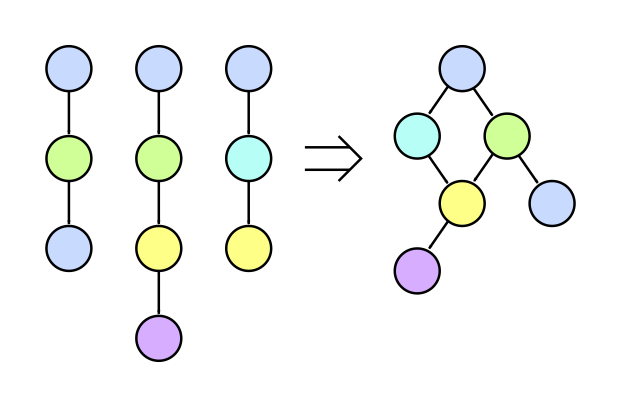
\includegraphics[width=0.9\textwidth]{res/naive-cyoa.pdf}
%\end{center}
%\end{frame}
%
%\begin{frame}{The Problem}
%\begin{itemize}
%  \item Where do you put the branches?
%  \item How many options should each branch have?
%  \item What outcomes should the different branches have?
%\end{itemize}
%%\pause
%%\begin{center}
%%How do choices affect the narrative?
%%\end{center}
%\end{frame}
%
%\begin{frame}{The Problem}
%\begin{itemize}
%  \item How do choices affect a narrative?
%\end{itemize}
%\end{frame}
%
%\begin{frame}{The Solution}
%  \itshape
%  ``By reasoning deliberately about choices \textbf{using a theory of choice poetics}, a generative narrative system can construct fixed-form branching narratives that give the player a feeling of agency which persists even when different branches of those narratives are explored.''
%\end{frame}
%
%\begin{frame}{The System}
%  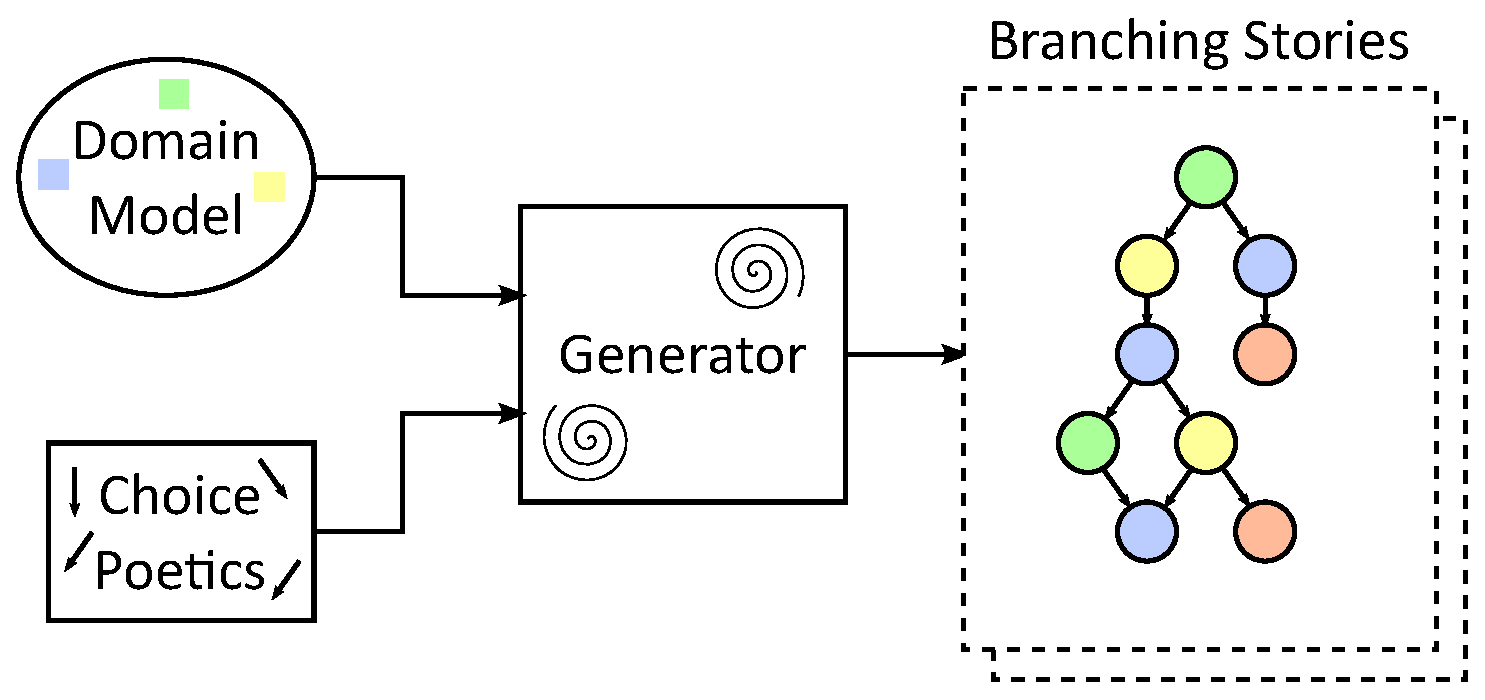
\includegraphics[width=0.9\textwidth]{res/high-level-architecture.eps}
%\end{frame}
%
%\begin{frame}{Outline}
%  \begin{itemize}
%    \item Related work
%    \item Choice poetics
%    \begin{itemize}
%      \item Modes of engagement
%      \item Choice idioms
%      \item Dimensions of player experience
%    \end{itemize}
%    \item More related work
%    \item Technical approach
%    \begin{itemize}
%      \item Story Domain
%      \item Generating narrative
%      \item Generating choices
%    \end{itemize}
%    \item Evaluation
%    \begin{itemize}
%      \item Empirical
%      \item Critical
%    \end{itemize}
%  \end{itemize}
%\end{frame}
%
%\begin{frame}{Outline}
%  \begin{itemize}
%    \item \textbf{Related work}
%    \item Choice poetics
%    \begin{itemize}
%      \item Modes of engagement
%      \item Choice idioms
%      \item Dimensions of player experience
%    \end{itemize}
%    \item More related work
%    \item Technical approach
%    \begin{itemize}
%      \item Story Domain
%      \item Generating narrative
%      \item Generating choices
%    \end{itemize}
%    \item Evaluation
%    \begin{itemize}
%      \item Empirical
%      \item Critical
%    \end{itemize}
%  \end{itemize}
%\end{frame}
%
%\begin{frame}{Narrative Theory: Poetics}
%  \begin{tabular}{C{0.45\textwidth} C{0.45\textwidth}}
%    \includegraphics[height=0.3\textwidth]{res/aristotle.jpg} &
%    \includegraphics[height=0.3\textwidth]{res/freytag.jpg} \\
%    Aristotle & Gustav Freytag \\
%    \work{Poetics} & \work{Technique of the Drama} \\
%    circa 335 B.C. & 1894 \\
%  \end{tabular}
%\end{frame}
%
%\begin{frame}{Narrative Theory: Structuralism}
%  \begin{tabular}{C{0.45\textwidth} C{0.45\textwidth}}
%    \includegraphics[height=0.3\textwidth]{res/propp.jpg} &
%    \includegraphics[height=0.3\textwidth]{res/barthes.jpg} \\
%    Vladimir Propp & Roland Barthes \\
%    \work{Morphology of the Folktale} & \work{An Introduction to the Structural Analysis of Narrative} \\
%    1928 & 1975 \\
%  \end{tabular}
%\end{frame}
%
%\begin{frame}{Narrative Theory: Effects}
%  \begin{tabular}{C{0.45\textwidth} C{0.45\textwidth}}
%    \includegraphics[height=0.3\textwidth]{res/iran-nejad.jpg} &
%    \includegraphics[height=0.3\textwidth]{res/green.jpg} \hspace*{2pt}
%    \includegraphics[height=0.3\textwidth]{res/brock.jpg} \\
%    Asghar Iran-Nejad & Melanie Green \& Timothy Brock \\
%    \work{Cognitive and Affective Causes of Interest and Liking} & \work{The Role of Transportation in the Persuasiveness of Public Narratives} \\
%    1987 & 2000 \\
%  \end{tabular}
%\end{frame}
%
%\begin{frame}{Narrative Theory: Hypertext}
%  \begin{tabular}{C{0.3\textwidth} C{0.3\textwidth} C{0.3\textwidth}}
%    \includegraphics[height=0.3\textwidth]{res/bernstein.jpg} &
%    \includegraphics[height=0.3\textwidth]{res/morgan.jpg} &
%    \includegraphics[height=0.3\textwidth]{res/tosca.jpg} \\
%    Mark Bernstein & Wendy Morgan & Susana Tosca\\
%    \work{Patterns of Hypertext} & \work{Heterotopics, Towards a Grammar of Hyperlinks} & \work{A Pragmatics of Links} \\
%    1998 & 1999 & 2000 \\
%  \end{tabular}
%\end{frame}
%
%\begin{frame}{Meaning in Games: Procedural Rhetoric}
%  \begin{tabular}{C{0.45\textwidth} C{0.45\textwidth}}
%    \includegraphics[height=0.3\textwidth]{res/bogost.jpg} &
%    \includegraphics[height=0.3\textwidth]{res/treanor.png} \\
%    Ian Bogost & Mike Treanor \\
%    \work{Persuasive Games} & \work{Investigating Procedural Expression and Interpretation in Videogames} \\
%    2007 & 2013 \\
%  \end{tabular}
%\end{frame}
%
%\begin{frame}{Meaning in Games: Operational Logics \& Agency}
%  \begin{table}[h]
%  \hspace*{-2em}
%  \centering
%  \begin{tabular}{C{0.5\textwidth} C{0.5\textwidth}}
%    \includegraphics[height=0.3\textwidth]{res/wardrip-fruin.jpg} \hspace*{2pt}
%    \includegraphics[height=0.3\textwidth]{res/mateas.jpg} &
%    \includegraphics[height=0.28\textwidth]{res/dow.jpg} \hspace*{2pt}
%    \includegraphics[height=0.28\textwidth]{res/sali.jpg} \\
%    Noah Wardrip-Fruin \& Michael Mateas & \ldots \& Steven Dow \& Serdar Sali \\
%    \work{Defining Operational Logics} & \work{Agency Reconsidered} \\
%    2009 & 2009
%  \end{tabular}
%  \end{table}
%\end{frame}
%
%\begin{frame}{Meaning in Games: Agency}
%  \begin{table}[h]
%  \centering
%  \begin{tabular}{C{0.45\textwidth} C{0.5\textwidth}}
%    \includegraphics[height=0.3\textwidth]{res/laurel.jpg} &
%    \includegraphics[height=0.3\textwidth]{res/murray.jpg} \\
%    Brenda Laurel & Janet Murray\\
%    \work{Toward the Design of a Computer-Based Interactive Fantasy System} &
%    \work{Hamlet on the Holodeck: The Future of Narrative in Cyberspace} \\
%    1986 & 1997
%  \end{tabular}
%  \end{table}
%\end{frame}
%
%\begin{frame}{Critique and Practice}
%  \begin{quote}
%    \slshape
%  This is not your typical brain-teasing adventure game -- it's a character-builder, a choose-your-own adventure where you don't just make decisions, you determine how your character feels about them and how they may affect those around him.
%  \end{quote}
%  \attrib{Matt Buckley, online review of \work{The Wolf Among Us}\footnote{\tiny \url{http://gamingtrend.com/2013/10/24/episode-one-imbues-faith-wolf-among-us/}}}
%\end{frame}
%
%\begin{frame}{Critique and Practice}
%  From the Choice of Games game design blog cateogry\footnote{\url{http://www.choiceofgames.com/category/blog/game-design/}}:
%  \begin{itemize}
%    \item 5 Rules for Writing Interesting Choices in Multiple-Choice Games
%    \item Make a ``Choice of'' Game Your Own: Authorial Intent in IF
%    \item By the Numbers: How to Write a Long Interactive Novel That Doesn’t Suck
%    \item 4 Common Mistakes in Interactive Novels
%  \end{itemize}
%\end{frame}
%
%\begin{frame}{Outline}
%  \begin{itemize}
%    \item Related work
%    \item \textbf{Choice poetics}
%    \begin{itemize}
%      \item Modes of engagement
%      \item Choice idioms
%      \item Dimensions of player experience
%    \end{itemize}
%    \item More related work
%    \item Technical approach
%    \begin{itemize}
%      \item Story Domain
%      \item Generating narrative
%      \item Generating choices
%    \end{itemize}
%    \item Evaluation
%    \begin{itemize}
%      \item Empirical
%      \item Critical
%    \end{itemize}
%  \end{itemize}
%\end{frame}
%
%\begin{frame}{Choice Poetics}
%  \includegraphics[width=\textwidth]{res/two-roads.jpg}
%\end{frame}
%
%\begin{frame}{Choice Poetics}
%  Choices consist of:
%  \begin{itemize}
%    \item Framing
%    \item Options
%    \item Outcomes
%  \end{itemize}
%\end{frame}
%
%\begin{frame}{Choice Poetics}
%  Choices consist of:
%  \begin{itemize}
%    \item Framing--how the choice is presented.
%    \item Options
%    \item Outcomes
%  \end{itemize}
%\end{frame}
%
%\begin{frame}{Choice Poetics}
%  Choices consist of:
%  \begin{itemize}
%    \item Framing--how the choice is presented.
%    \item Options--the alternatives available to the player.
%    \item Outcomes
%  \end{itemize}
%\end{frame}
%
%\begin{frame}{Choice Poetics}
%  Choices consist of:
%  \begin{itemize}
%    \item Framing--how the choice is presented.
%    \item Options--the alternatives available to the player.
%    \item Outcomes--what happens afterwards.
%  \end{itemize}
%\end{frame}
%
%\begin{frame}{Choice Poetics}
%  \includegraphics[width=\textwidth]{res/two-roads.jpg}
%\end{frame}
%
%\begin{frame}{Choice Poetics: Overview}
%  \begin{itemize} 
%    \item Modes of Engagement
%    \item Choice Idioms
%    \item Dimensions of Experience
%  \end{itemize} 
%\end{frame}
%
%\begin{frame}{Choice Poetics: Overview}
%  \begin{itemize} 
%    \item Modes of Engagement--How players approach choices
%    \item Choice Idioms
%    \item Dimensions of Experience
%  \end{itemize} 
%\end{frame}
%
%\begin{frame}{Choice Poetics: Overview}
%  \begin{itemize} 
%    \item Modes of Engagement--How players approach choices
%    \item Choice Idioms--Specific choice structures and their effects
%    \item Dimensions of Experience
%  \end{itemize} 
%\end{frame}
%
%\begin{frame}{Choice Poetics: Overview}
%  \begin{itemize} 
%    \item Modes of Engagement--How players approach choices
%    \item Choice Idioms--Specific choice structures and their effects
%    \item Dimensions of Experience--Things that choice structures affect
%  \end{itemize} 
%\end{frame}
%
%\begin{frame}{Modes of Engagement}
%  \includegraphics[width=\textwidth]{res/scan-book.jpg}
%\end{frame}
%
%\begin{frame}{Modes of Engagement}
%  \begin{itemize}
%    \item Avatar play
%    \item Role play
%    \item Power play
%    \item Exploratory play
%    \item Analytical play
%    \item Critical play
%    \item etc.
%  \end{itemize}
%\end{frame}
%
%\begin{frame}{Modes of Engagement: Avatar Play}
%  \includegraphics[width=\textwidth]{res/avatar-play.jpg}
%\end{frame}
%
%\begin{frame}{Modes of Engagement: Role Play}
%  \includegraphics[width=\textwidth]{res/renfaire.jpg}
%\end{frame}
%
%\begin{frame}{Modes of Engagement: Power Play}
%  \begin{center}
%    \includegraphics[height=0.7\textheight]{res/timmy.jpg}
%  \end{center}
%\end{frame}
%
%\begin{frame}{Modes of Engagement: Exploratory Play}
%  \begin{center}
%    \includegraphics[height=0.7\textheight]{res/exploratory-play.jpg}
%  \end{center}
%\end{frame}
%
%\begin{frame}{Modes of Engagement: Analytical Play}
%  \begin{center}
%    \includegraphics[height=0.8\textheight]{res/chimneyrock.png}
%  \end{center}
%\end{frame}
%
%\begin{frame}{Modes of Engagement: Critical Play}
%  \begin{center}
%    \includegraphics[height=0.8\textheight]{res/alice-in-park.jpg}
%  \end{center}
%\end{frame}
%
%\begin{frame}{Modes of Engagement: Example}
%  \includegraphics[width=\textwidth]{res/me-choice-brighter.png}
%\end{frame}
%
%\begin{frame}{Choice Idioms}
%  \begin{itemize}
%    \item Dilemma
%    \item Flavor choice
%    \item Blind choice
%    \item etc.
%  \end{itemize}
%\end{frame}
%
%\begin{frame}{Choice Idioms: (Di)lemma}
%  \includegraphics[width=\textwidth]{res/starter-pokemon.png}
%\end{frame}
%
%\begin{frame}{Choice Idioms: Flavor Choice}
%  \includegraphics[width=\textwidth]{res/da-customization.jpg}
%\end{frame}
%
%\begin{frame}{Choice Idioms: Blind Choice}
%  \includegraphics[width=\textwidth]{res/megaman2-difficulty.png}
%\end{frame}
%
%\begin{frame}{Dimensions of Experience}
%  \begin{itemize}
%    \item Agency
%    \item Absorption
%    \item Regret
%    \item etc.
%  \end{itemize}
%\end{frame}
%
%\begin{frame}{Dimensions of Experience: Agency}
%  \includegraphics[width=\textwidth]{res/doom-screenshot.jpg}
%\end{frame}
%
%\begin{frame}{Dimensions of Experience: Absorption}
%  \includegraphics[width=\textwidth]{res/absorbed-player.jpg}
%\end{frame}
%
%\begin{frame}{Dimensions of Experience: Regret}
%  \includegraphics[width=\textwidth]{res/twd-regret.jpg}
%\end{frame}
%
%\begin{frame}{Choice Poetics}
%  \color{black} $\rightarrow$ A framework for understanding the narrative effects of choices. \\
%  \pause
%  \begin{center}
%  (this work is only an outline)
%  \end{center}
%\end{frame}
%
%\begin{frame}{Outline}
%  \begin{itemize}
%    \item Related work
%    \item Choice poetics
%    \begin{itemize}
%      \item Modes of engagement
%      \item Choice idioms
%      \item Dimensions of player experience
%    \end{itemize}
%  \item \textbf{More related work}
%    \item Technical approach
%    \begin{itemize}
%      \item Story Domain
%      \item Generating narrative
%      \item Generating choices
%    \end{itemize}
%    \item Evaluation
%    \begin{itemize}
%      \item Empirical
%      \item Critical
%    \end{itemize}
%  \end{itemize}
%\end{frame}
%
%%\begin{frame}{Computational Narrative: History}
%%  \begin{itemize}
%%    \item Klein 1971
%%    \item Meehan 1976
%%    \item Dehn 1981
%%    \item Lebowitz 1984
%%  \end{itemize}
%%\end{frame}
%%
%%\begin{frame}{Computational Narrative: History}
%%  \begin{itemize}
%%    \item Klein 1971--Monte Carlo storytelling
%%    \item Meehan 1976
%%    \item Dehn 1981
%%    \item Lebowitz 1984
%%  \end{itemize}
%%\end{frame}
%%
%%\begin{frame}{Computational Narrative: History}
%%  \begin{itemize}
%%    \item Klein 1971--Monte Carlo storytelling
%%    \item Meehan 1976--recursive character plans
%%    \item Dehn 1981
%%    \item Lebowitz 1984
%%  \end{itemize}
%%\end{frame}
%%
%%\begin{frame}{Computational Narrative: History}
%%  \begin{itemize}
%%    \item Klein 1971--Monte Carlo storytelling
%%    \item Meehan 1976--recursive character plans
%%    \item Dehn 1981--author-level planning
%%    \item Lebowitz 1984
%%  \end{itemize}
%%\end{frame}
%%
%%\begin{frame}{Computational Narrative: History}
%%  \begin{itemize}
%%    \item Klein 1971--Monte Carlo storytelling
%%    \item Meehan 1976--recursive character plans
%%    \item Dehn 1981--author-level planning
%%    \item Lebowitz 1984--author and character plans
%%  \end{itemize}
%%\end{frame}
%
%\begin{frame}{Author-Level Systems}
%  \begin{itemize}
%    \item \work{Minstrel} (Turner 1993)--CBR and author-level planning
%    \item \work{Mexica} (P\'erez y P\'erez \& Sharples 2001)--Also used CBR along with a separate reflection phase
%  \end{itemize}
%  \hrule
%  \begin{itemize}
%    \item Along with Brandon Tearse, Michael Mateas, and Noah Wardrip-Fruin I've helped reconstruct \work{Minstrel} as \work{Skald}.
%    \item My high-level architecture is based on these systems.
%  \end{itemize}
%\end{frame}
%
%%\begin{frame}{Computational Narrative: Modern Systems}
%%  Non-interactive:
%%  \begin{itemize}
%%    \item Riedl \& Young 2004--Partial order causal link planning
%%    \item Theune et al. 2003--Intelligent agents
%%    \item Gerv\'as et al. 2005--Case-based reasoning
%%    \item Zhu \& Onta\~n\'on 2010--Computational analogy
%%    \item Bui et al. 2010--Genetic algorithms
%%    \item Li et al. 2013--Crowdsourced plot graphs
%%  \end{itemize}
%%  Interactive:
%%  \begin{itemize}
%%    \item Sgouros et al. 1996--Agent-driven
%%    \item Cavazza et al. 2002--Hierarchical task network planning
%%    \item Aylett et al. 2005--Emotional agents
%%  \end{itemize}
%%\end{frame}
%
%\begin{frame}{Drama Management}
%  \begin{itemize}
%    \item \work{Tea for Three}/\work{Moe} (Weyhrauch 1997)--Original concept
%    \item \work{Fa\c{c}ade}/\work{ABL} (Mateas \& Stern 2002)--Dramatic beats
%    \item \work{PaSSAGE} (Thue et al. 2007)--Player modelling
%  \end{itemize}
%  \hrule
%  \begin{itemize}
%    \item Drama managers maximize the use of fixed content in the face of player choice by manipulating outcomes.
%    \item A branching story generator creates a range of outcomes to support player choice.
%  \end{itemize}
%\end{frame}
%
%\begin{frame}{Narrative Phenomena}
%  \begin{itemize}
%    \item \work{Suspenser} Cheong \& Young 2006--Suspense
%    \item \work{Prevoyant} Bae \& Young 2008--Flashback/foreshadowing
%    \item \work{INFER} Niehaus \& Young 2009--Salience and inferences
%  \end{itemize}
%  \hrule
%  \begin{itemize}
%    \item These systems model specific cognitive phenomena
%    \item They all focus on discourse generation alone
%  \end{itemize}
%\end{frame}
%
%\begin{frame}{Choice Idioms}
%  \begin{itemize}
%    \item Barber \& Kudenko 2007--Dillema-driven interactive narrative
%  \end{itemize}
%  \hrule
%  \begin{itemize}
%    \item A single choice idiom as the basis of a story generation strategy
%  \end{itemize}
%\end{frame}
%
%\begin{frame}{Illusory Agency}
%  \begin{itemize}
%    \item Thue et al. 2011--Perception of agency
%    \item Fendt et al. 2012--Illusion of ``agency''
%  \end{itemize}
%  \hrule
%  \begin{itemize}
%    \item After a single playthrough, players use heuristics to estimate how much agency is available
%    \item Certain kinds of choices are perceived as higher-agency than others (if the player only knows one of the outcomes)
%    \item Explicitly acknowledging player choices makes players think that those choices are weighty
%  \end{itemize}
%\end{frame}
%
%\begin{frame}{Choice Acknowledgment}
%\begin{center}
%  \vspace*{-5pt}
%  \includegraphics[width=0.95\textwidth]{res/clem-will-remember.jpg}
%\end{center}
%\end{frame}
%
%\begin{frame}{Outline}
%  \begin{itemize}
%    \item Related work
%    \item Choice poetics
%    \begin{itemize}
%      \item Modes of engagement
%      \item Choice idioms
%      \item Dimensions of player experience
%    \end{itemize}
%    \item More related work
%    \item \textbf{Technical approach}
%    \begin{itemize}
%      \item Story Domain
%      \item Generating narrative
%      \item Generating choices
%    \end{itemize}
%    \item Evaluation
%    \begin{itemize}
%      \item Empirical
%      \item Critical
%    \end{itemize}
%  \end{itemize}
%\end{frame}
%
%\begin{frame}{My Thesis}
%  \itshape
%``By reasoning deliberately about choices using a theory of choice poetics, a generative narrative system can construct fixed-form branching narratives that give the player a feeling of agency which persists even when different branches of those narratives are explored.''
%\end{frame}
%
%\begin{frame}{The Goal}
%  \color{black} $\rightarrow$ A system that generates branching stories with robust agency.
%\end{frame}
%
%\begin{frame}{Story Domain}
%  \begin{columns}[T]
%    \begin{column}{.6\textwidth}
%      \begin{block}{}
%\work{One Thousand and One Nights} is a collection of Middle-Eastern folk-tales.
%\begin{itemize}
%  \item It represents a coherent story corpus with a consistent sytle.
%  \item \work{Tales of the Arabian Nights} is a story board game with a similar setting which includes choices.
%  \item \work{Twist of Fate} is a branching narrative with a similar setting.
%  \item It contains strong themes and conventional structures that can be exploited.
%\end{itemize}
%      \end{block}
%    \end{column}
%    \begin{column}{.4\textwidth}
%      \begin{block}{}
%\includegraphics[height=0.8\textheight]{res/1001nights-illustration.jpg}
%      \end{block}
%    \end{column}
%  \end{columns}
%\end{frame}
%
%\begin{frame}{High-Level Architecture}
%  \begin{itemize}
%    \item Use reactive planning to pursue interacting author goals.
%    \item Independent plans will communicate via a blackboard.
%    \pause
%    \item Four author goal categories:
%    \begin{enumerate}
%      \item Seed goals
%      \item Construction goals
%      \item Coherence goals
%      \item Choice structure goals
%    \end{enumerate}
%  \end{itemize}
%\end{frame}
%
%\begin{frame}{Story Representation}
%  \begin{itemize}
%    \item Stories will be represented using logical predicates.
%    \item Plans will use answer set programming to operate on story elements.
%    \item Text will be generated using a dedicated solution such as \work{Curveship}\footnote{Montfort 2009}.
%  \end{itemize}
%\end{frame}
%
%\begin{frame}{Generation Example}
%  \includegraphics[height=0.8\textheight]{res/system_demo.eps}
%\end{frame}
%
%\begin{frame}{Generating Choices}
%  \begin{itemize}
%    \item Assume avatar play as the mode of engagement.
%    \item Reason about framing, options, and outcomes.
%    \item Focus only on agency for now.
%  \end{itemize}
%\end{frame}
%
%\begin{frame}{Leveraging Choice Poetics}
%  \begin{itemize}
%    \item An encoding of genre expectations:
%      \begin{itemize}
%        \item Option expectations
%        \item Outcome expectations
%      \end{itemize}
%    \item Heuristics for agency:
%      \begin{itemize}
%        \item Presence of all expected options
%        \item Lack of violation of expected outcomes
%      \end{itemize}
%    \item Predictability can be avoided as long as situations commonly generate more than one expected outcome.
%    \pause
%    \item The theory of choice poetics is still under development.
%      \begin{itemize}
%        \item Identify choice idioms linked with agency
%      \end{itemize}
%  \end{itemize}
%\end{frame}
%
%\begin{frame}{Outline}
%  \begin{itemize}
%    \item Related work
%    \item Choice poetics
%    \begin{itemize}
%      \item Modes of engagement
%      \item Choice idioms
%      \item Dimensions of player experience
%    \end{itemize}
%    \item More related work
%    \item Technical approach
%    \begin{itemize}
%      \item Story Domain
%      \item Generating narrative
%      \item Generating choices
%    \end{itemize}
%  \item \textbf{Evaluation}
%    \begin{itemize}
%      \item Empirical
%      \item Critical
%    \end{itemize}
%  \end{itemize}
%\end{frame}
%
%\begin{frame}{Research Question}
%  \color{black} $\rightarrow$ Does a theory of choice poetics enable the construction of a generator that can produce branching narratives which provide agency that is robust to replay?
%\end{frame}
%
%\begin{frame}{Robust Agency}
%  \begin{itemize}
%    \item Wardrip-Fruin et al. 2009--Agency as informed control over a system
%    \item Theune et al. 2011 and Fendt et al. 2012--The illusion of agency
%    \item Mitchell 2012--Rereading for closure
%  \end{itemize}
%  \hrule
%  \begin{itemize}
%    \item Can we provide ``real'' agency?
%    \item Real agency would stand up to multiple playthroughs.
%  \end{itemize}
%\end{frame}
%
%\begin{frame}{Empirical Evaluation}
%  \begin{itemize}
%    \item Use and augment existing survey tools to measure agency
%    \item Measure agency both after one playthrough and after several
%    \item Compare a ``false agency'' version of the system with a version that strives for robust agency
%  \end{itemize}
%\end{frame}
%
%\begin{frame}{Study Design}
%  \begin{tabular}{C{0.3\textwidth} C{0.35\textwidth} C{0.35\textwidth}}
%    & \textbf{False agency} & \textbf{Robust agency} \\
%    \textbf{Branches} & always binary & multiple-option \\
%    \textbf{Outcomes} & similar states & divergent states \\
%    \textbf{Acknowledgement} & explicit--shallow & implicit--deep \\
%  \end{tabular}
%  \vspace{2em}
%  \begin{itemize}
%    \item The false agency case mimicks the conditions in Fendt et al.
%  \end{itemize}
%\end{frame}
%
%\begin{frame}{Control Cases}
%  \begin{enumerate}
%    \item Baseline case will ignore genre information and generate choices randomly
%    \item Include a version that adds choice acknowledgement to the robust agency case
%    \item To see whether the system performs well, include a case where a human controls the choices
%      \begin{itemize}
%        \item Have an expert human branching story author tell the system what choices to use and what their outcomes should be like
%        \item The system will still generate the narrative content
%      \end{itemize}
%  \end{enumerate}
%\end{frame}
%
%\begin{frame}{Critical Evaluation}
%  Artistic output should be evaluated using techniques commonly applied to art (Zhu 2012).
%  \pause
%  \begin{itemize}
%    \item Contact experienced authors of branching and/or computational narrative.
%    \item Ask for critiques of both individual stories and of the system as a whole.
%    \item These critiques will be more useful for system development than an empirical evaluation.
%  \end{itemize}
%\end{frame}
%
%\begin{frame}{Schedule}
%
%  \tiny
%\begin{tabular}{r l p{2in}}
%\toprule
%Year & Quarter & Items \\
%\midrule \addlinespace[0.5em]
%2014 & Winter & Theory development and genre analysis. \\ \addlinespace[0.5em]
%     & Spring & Continue theory development and begin work on prototype. \\ \addlinespace[0.5em]
%     & Summer & Possible internship or continue work on theory \& prototype. \\ \addlinespace[0.5em]
%     & Fall & Write a choice poetics paper focusing on agency; complete first prototype system. \\ \addlinespace[0.5em] \midrule \addlinespace[0.6em]
%2015 & Winter & Begin work on final system (theory development is now driven by the implementation). \\ \addlinespace[0.5em]
%     & Spring & Start finalizing the system in preparation for evaluation. \\ \addlinespace[0.5em]
%     & Summer & Finalize generative system for evaluation; run pilot study. \\ \addlinespace[0.5em]
%     & Fall & Write a paper about the system; run qualitative study and gather critiques; begin writing dissertation. \\ \addlinespace[0.5em] \midrule \addlinespace[0.6em]
%2016 & Winter & Analyze results and continue writing dissertation. \\ \addlinespace[0.5em]
%     & Spring & Finish and defend dissertation. \\ \addlinespace[0.5em]
%\bottomrule
%\end{tabular}
%\end{frame}
%
%\begin{frame}{Questions?}
%  \begin{itemize}
%    \item Related work
%    \item Choice poetics
%    \begin{itemize}
%      \item Modes of engagement
%      \item Choice idioms
%      \item Dimensions of player experience
%    \end{itemize}
%    \item More related work
%    \item Technical approach
%    \begin{itemize}
%      \item Story Domain
%      \item Generating narrative
%      \item Generating choices
%    \end{itemize}
%  \item Evaluation
%    \begin{itemize}
%      \item Empirical
%      \item Critical
%    \end{itemize}
%  \end{itemize}
%\end{frame}

\end{document}
